\section{Entorno de desarrollo}\label{sec:entorno}

\subsection*{Visual Studio Code}

El entorno recomendado\footnote{Lean también tiene soporte mediante plugins para
	los editores \textit{emacs} y \textit{vim}.} para desarrollar código
\textit{Lean} es el editor \textit{Visual Studio Code}\footnote{Aconsejamos
	utilizar la distribución de \textit{Visual Studio Code} de software libre,
	\href{https://vscodium.com/}{VSCodium}.}. En este editor, una vez instalado el
plugin que da soporte a \textit{Lean}, tenemos acceso a una serie de
herramientas que facilitan la lectura y desarrollo de código en Lean. A
continuación exponemos alguna de estas herramientas.

\subsection*{Consulta de tipos}

Moviendo el cursor por encima de definiciones o tácticas podemos obtener
información adicional sobre un término, tipo o táctica, accediendo a su tipo, su
definición o la documentación correspondiente.

\subsection*{Símbolos matemáticos}

Como se ha mencionado anteriormente en este documento, en \textit{Lean} se
pueden utilizar símbolos unicode para expresar tipos útiles en la formalización
de matemáticas y obtener así un código más cercano a las notaciones lógicas a
las que estamos acostumbrados a usar en matemáticas.

La inclusión de estos caracteres está facilitada en el entorno de desarrollo,
escribiendo comandos que empiecen por \texttt{\textbackslash} estos se
reemplazarán por el caracter correspondiente. Por ejemplo al escribir
\texttt{\textbackslash to} este comando se reemplazará automáticamente por el
caracter \lstinline{→}, \texttt{\textbackslash lambda} por \lstinline{λ} y
\texttt{\textbackslash N} por \lstinline{ℕ}. Si mantenemos el cursor encima de
un símbolo, un panel informativo nos indicará el código que podemos utilizar
para escribirlo.

\subsection*{Panel de estado táctico}

La herramienta más importante de este entorno es el panel lateral desde el cual
podemos consultar el estado táctico. En la siguiente captura de pantalla se ve
cómo, situando el cursor en un paso de una demostración, el panel lateral
proporciona toda la información contextual del estado táctico correspondiente.

\begin{figure}[htbp]
	\centerline{\frame{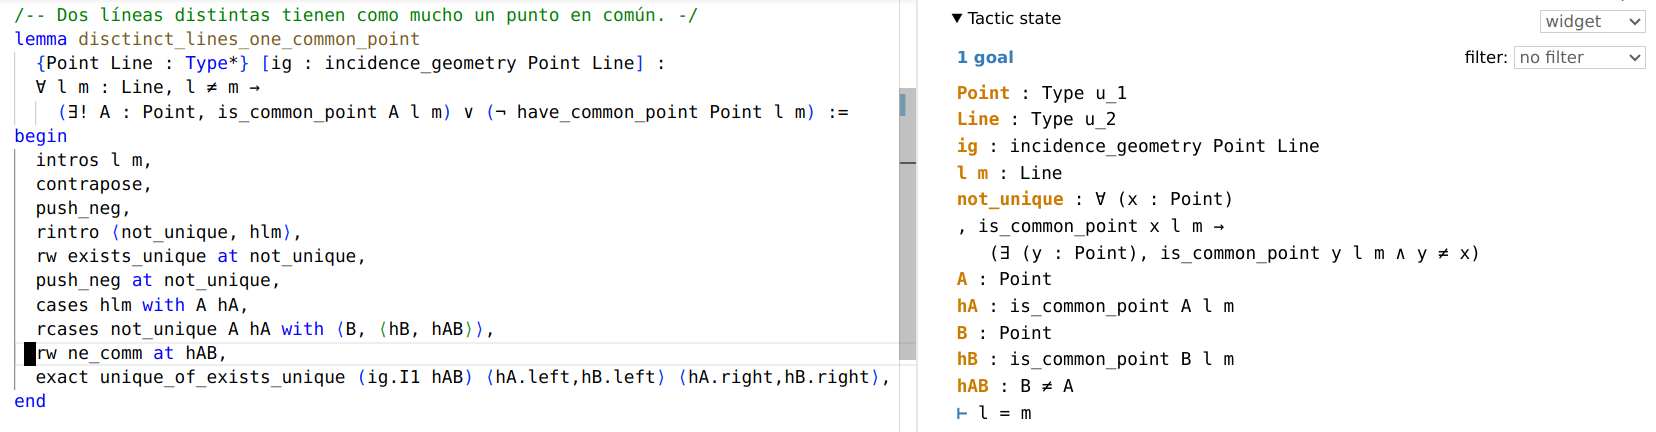
\includegraphics[width=17cm]{./imgs/captura.png}}}
	\caption*{Captura de pantalla del entorno de dearrollo en el editor \textit{Visual Studio Code}.}
	\label{figure:entorno}
\end{figure}

Durante la formalización o lectura de una demostración en \textit{Lean} estamos
continuamente moviéndonos a través del código y observando de qué forma varía el
estado táctico.


